\documentclass[%
  border=1mm
%  border={0pt 0pt 0pt 0pt} % left bottom right top
]{standalone}% http://ctan.org/pkg/standalone

\usepackage{tikz}

% packages we need for platform detection
\usepackage{pdftexcmds}
\usepackage{catchfile}
\usepackage{ifluatex}
\usepackage{ifplatform}
\usepackage{fontspec}
\iflinux
\setmainfont{Roboto}
\setsansfont{Roboto}
\else
\setmainfont{PT Sans}
\setsansfont{PT Sans}
\fi


%\usepackage[defaultsans]{droidsans}
%\renewcommand*\familydefault{\sfdefault} %% Only if the base font of the document is to be typewriter style
%\usepackage[T1]{fontenc}

\newcommand\centerdrillmark{} % just for safety
\def\centerdrillmark{
  \draw [dashed] (0,2.5mm) -- (0,-2.5mm);
	\draw [dashed]  (2.5mm,0) -- (-2.5mm,0);
}

\begin{document}

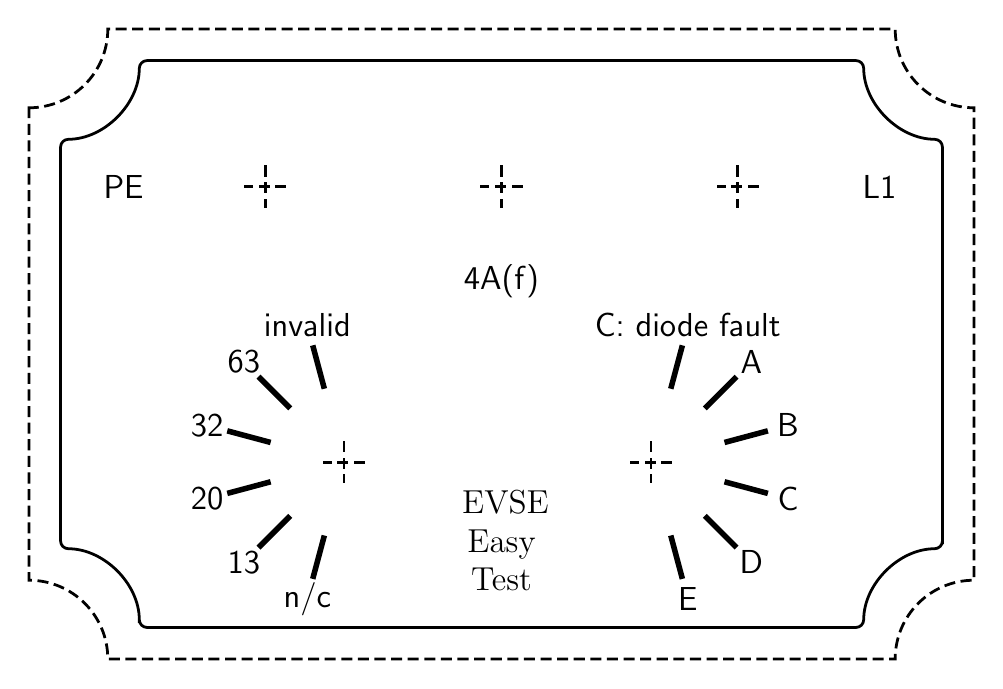
\begin{tikzpicture}[line cap=rect,line width=1pt]

% Bopla ET-215 frame: Outer dimensions
\draw [dashed] (0mm,70mm) arc[radius=10mm, start angle=-90, end angle=0] --
	(110mm,80mm) --
	(110mm,80mm) arc[radius=10mm, start angle=180, end angle=270] --
	(120mm,10mm) --
	(120mm,10mm) arc[radius=10mm, start angle=90, end angle=180] --
	(10mm,0mm) --
	(10mm,0mm) arc[radius=10mm, start angle=0, end angle=90] --
	cycle;
% Cutline for top of housing
\draw [color=black, rounded corners=1mm] (4mm,66mm) arc[radius=10mm, start angle=-90, end angle=0] --
	(104mm,76mm) --
	(106mm,76mm) arc[radius=10mm, start angle=180, end angle=270] --
	(116mm,14mm) --
	(116mm,14mm) arc[radius=10mm, start angle=90, end angle=180] --
	(14mm,4mm) --
	(14mm,4mm) arc[radius=10mm, start angle=0, end angle=90] --
	cycle;


% Product name
\begin{scope}[shift={(60mm,15mm)}]
	\node[align=center, font=\large, text width=10mm] at (0:0mm)
	{\textsf\textbf{{EVSE Easy Test}}};
\end{scope}

% PE switch
\begin{scope}[shift={(30mm,60mm)}]
	\centerdrillmark;
	\node[font=\large] at (180:18mm) {\textsf{PE}};
\end{scope}

% Fuse
\begin{scope}[shift={(60mm,60mm)}]
	\centerdrillmark;
	\node[font=\large] at (270:12mm) {\textsf{4A(f)}};
\end{scope}

% L1 LED
\begin{scope}[shift={(90mm,60mm)}]
	\centerdrillmark
	\node[font=\large] at (0:18mm) {\textsf{L1}};
\end{scope}


% State dial
\begin{scope}[shift={(79mm,25mm)}]
	%\draw (0,0) circle [radius=13.1mm];
	\centerdrillmark
	\foreach \angle/\label [count=\xi] in 
	{
		75/{C: diode fault},45/A,15/B,-15/C,-45/D,-75/E
	}
	{
		\draw[line width=2pt] (\angle:10mm) -- (\angle:15mm);
		\node[font=\large] at (\angle:18mm) {\textsf{\label}};
	}
\end{scope}

% Max current dial
\begin{scope}[shift={(40mm,25mm)}]
	%\draw (0,0) circle [radius=13.1mm];
	\centerdrillmark
	\foreach \angle/\label [count=\xi] in
	{
		180-75/invalid,180-45/63,180-15/32,180+15/20,180+45/13,180+75/{n/c}
	}
	{
		\draw[line width=2pt] (\angle:10mm) -- (\angle:15mm);
		\node[font=\large] at (\angle:18mm) {\textsf{\label}};
	}
\end{scope}



\end{tikzpicture}

\end{document}
